\section{Data Quality}%
\label{sec:data_quality}

One of the most important ingredients for training large `foundation' models is data.
Having access to a large amount of data is, however, insufficient; in fact, the \emph{quality} of the data also has a strong effect on the model's behavior.
For 3D reconstruction, we found that noisy data introduces particular failure modes in both self-supervised and supervised training.

For self-supervised training, we observe that unreasonably difficult videos, such as the ones containing discontinuous shot transitions as commonly seen in television footage, induce sharp loss spikes and may cause gradients to explode, resulting in a degradation of the model's performance.
We therefore restrict self-supervised training to videos that pass the VLM pre-filtering check of \cref{sec:annotation-pipeline}, which reliably removes such cases.

In the supervised stage, the effects of noisy data are more subtle but equally important.
We find that different types of errors in the annotations translate into specific failure modes at inference time.
What is worse, these failure modes do not affect most of the images in standard benchmarks and may thus not be detected in the quantitative results.
Instead, they emerge only when the model is tested on a new sample that resembles an incorrectly labeled sample seen during training.
This behavior indicates that, while the model does learn the general principles of 3D reconstruction, it can nevertheless memorize idiosyncratic noise as well.
Next, we discuss the most representative cases we have encountered.

\begin{figure}
\centering
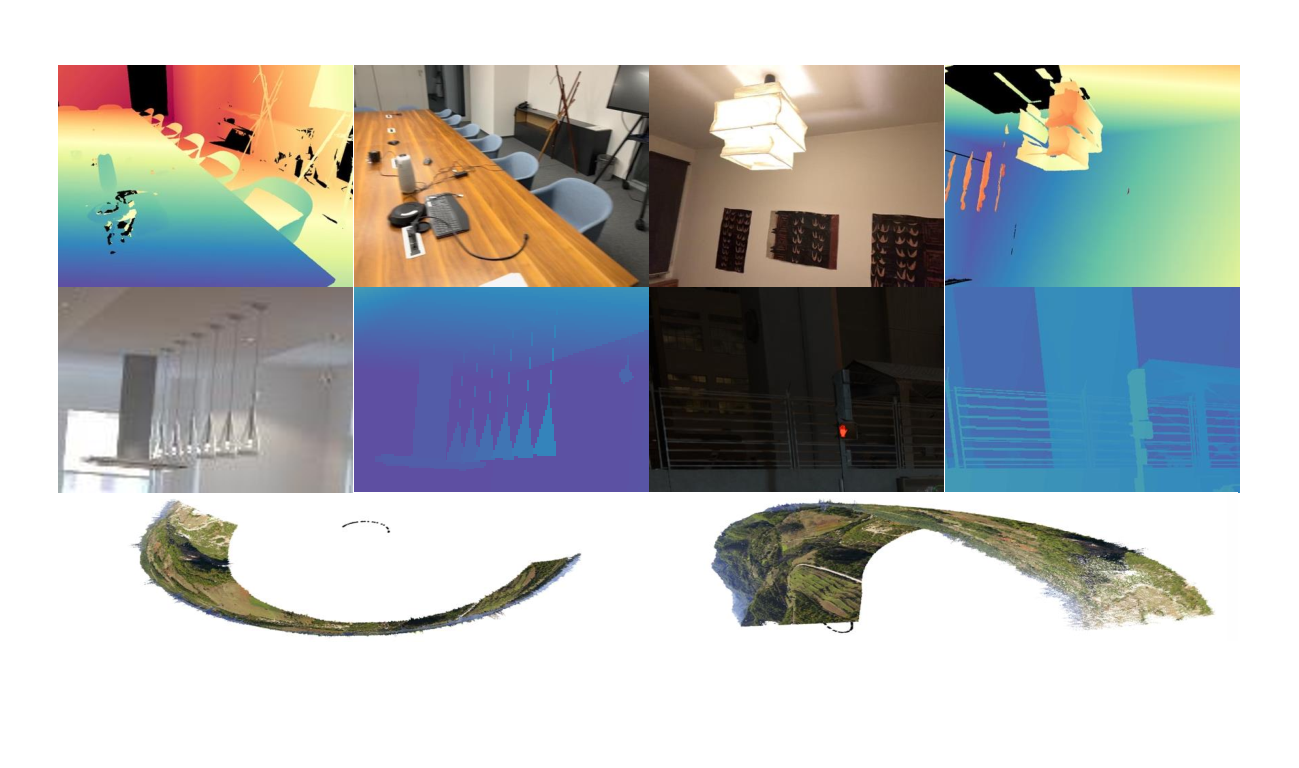
\includegraphics[width=0.95\linewidth]{figures/data_v3.pdf}
\caption{\textbf{Common Data Issues.}
Top: examples from ScanNet++.
Middle: examples from synthetic datasets such as Hypersim.
Bottom: the doming effect.}%
\label{fig:data_quality}
\vspace{-8pt}
\end{figure}




\paragraph{Sensors.}

Some datasets annotate real-world scenes using sensors such as LiDAR or depth cameras.
A common failure mode here is foreground-background leakage.
For example, as shown in the top row of~\cref{fig:data_quality} with an example from ScanNet++, the depth of the chair's back corresponds to the background floor or wall, likely due to misalignment or holes in the sensor capture.
We also observe spurious depth artifacts around the hanging light fixture, where the rendered depth contains fragmented foreground structures that do not correspond to the visible lamp geometry.
Such artifacts are likely caused by unreliable sensor capture or reconstruction around over-exposed and partially translucent objects.
We therefore exclude such datasets in the later phase of training.

\paragraph{Thin Structure.}

Synthetic data usually provides more accurate geometric annotations, but thin structures can be inaccurate in some synthetic datasets too.
Objects such as fence bars often occupy only a few pixels and lie on sharp depth discontinuities.
Although these structures are clearly visible in the RGB image, their rendered depth can be incomplete, overly smoothed, or misaligned.
As a result, the label may assign a thin structure to the depth of the wall, window, floor, or distant background behind it, rather than to the actual object surface, as shown in the middle row of~\cref{fig:data_quality}.
At inference time, the model may ignore thin objects, recover only their thicker or lower parts, or produce depth maps in which thin structures are washed out by nearby large surfaces.
This is a common problem in existing models, and we hypothesize that it can be mitigated with higher-resolution inputs or better synthetic data.

\paragraph{Fake Background.}

Another common issue in synthetic data is fake background.
For example, in Kubric, PointOdyssey, BEDLAM, the background depth may correspond to proxy dome or floor geometry used for HDRI rendering, rather than the true 3D structure suggested by the appearance of the background.
Although this is reasonable for rendering, it provides depth values that are inconsistent with the scene semantics.
For datasets with a clear boundary between the real foreground and the synthetic background, such as BEDLAM, we filter out the background during training by thresholding the maximum valid foreground depth.
We exclude the remaining from training.

\paragraph{Doming Effect.}

Methods using bundle adjustment, such as COLMAP~\cite{schonberger16structure-from-motion}, MegaSaM~\cite{li25megasam:}, and ViPE~\cite{huang25vipe:}, can be used to generate pseudo ground truth.
However, care is needed because they may produce degenerate solutions such as the doming effect, as shown in the bottom row of~\cref{fig:data_quality}.
This usually arises from weak global constraints in the image collection, \eg, near-parallel viewing directions, insufficient loop closure, small triangulation angles, or inaccurate camera self-calibration, especially radial-distortion errors, which are common in Internet videos.
Under these conditions, bundle adjustment can still achieve a low reprojection error while bending the recovered cameras and scene geometry into a globally inconsistent curved shape.
Such reconstructions may appear locally plausible but provide incorrect large-scale geometry, making them harmful as supervision.
They can be filtered out by supervised geometric filtering, as discussed in~\cref{sec:data}, or by comparing the annotated depths with predictions from existing monocular depth models or feed-forward reconstruction models.

\paragraph{Humans in Walls.}

We observe a recurring failure case in near-static street-view videos with pedestrians moving through the scene: almost all existing feed-forward reconstruction models often absorb humans into the static background, estimating them as part of nearby walls or buildings.
This failure appears to be related to ambiguous boundary pixels in existing training datasets.
For example, the most widely used multiview dataset Megadepth was annotated with COLMAP on phototourism images that often contain people.
At human boundaries, the patch match stereo algorithm may assign some pixels to the surrounding static architecture, causing supervision to treat parts of people as background.
Excluding MegaDepth or re-estimating its depths can substantially reduce this artifact.

\paragraph{Data Ambiguities.}

Inconsistencies in annotations across different datasets can lead to confusing model behaviors.
For instance, in synthetic datasets such as Aria Synthetic Environments and HyperSim, outdoor scenes are often rendered as 2D textures applied to windows, meaning the GT depth corresponds to the window surface itself.
Conversely, in other datasets, depth values correctly represent the actual physical objects visible through windows.
This inherent GT mismatch across the training corpus confuses the model, which occasionally leads to strange predictive behaviors.

Several recent datasets have introduced alternative pipelines for annotating Internet videos, including SceneScribe-1M~\cite{wang26scenescribe-1m:}, PointWorld~\cite{huang26pointworld:}, Sekai~\cite{li25sekai:}, SpatialVID~\cite{wang25spatialvid:}, and OmniWorld~\cite{zhou26omniworld:}, which may also be worth exploring.




